\chapter{热力学平衡与开口系统}\label{ch:b2:open-systems}

本科一年级分册中的热力学讨论的是封闭系统——
圆筒中一定质量的气体，被压缩、加热、膨胀。但
真正给房屋供暖、为食物制冷、产生电能的机器，
都有一股\emph{流}穿过：蒸汽以每秒数百千克的速率
流过发电厂的涡轮机，制冷剂在热泵的压缩机、冷凝器、
膨胀阀和蒸发器中循环，空气流过喷气发动机的压缩机
和燃烧室。每个部件都是一个\emph{开口系统}，即物质
进入和离开的一块空间区域，热力学第一定律和第二定律
必须针对它重新表述。重新表述并不复杂——
关键在于，被推入系统的流体除内能外，
还携带着把它推入时所做的功，
这正是为什么对流动而言，自然的能量量度是\emph{焓}，
而非内能。
本章建立稳定流动开口系统的质量、能量和熵的平衡，
将其应用于基本部件——
喷管、节流阀、压缩机、涡轮机、换热器——并将这些部件
组合成周末问题所估算的两个循环：
热泵与蒸汽动力装置。

\begin{omfigure}
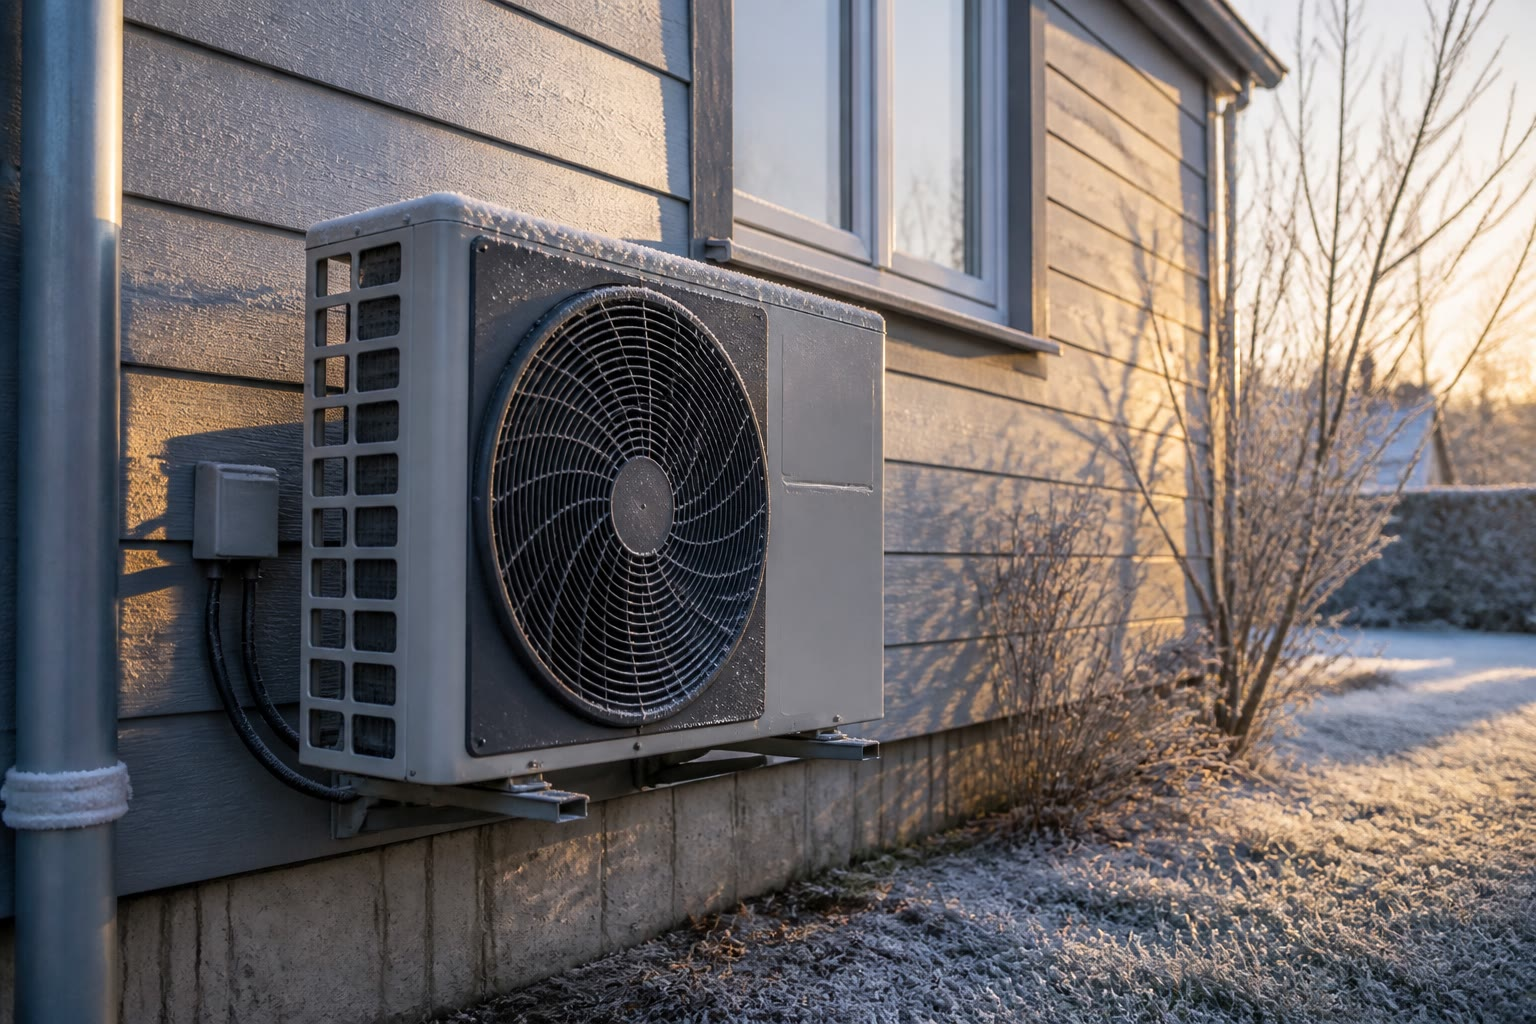
\includegraphics[width=0.58\linewidth]{images/book4/ai/b4-27-heat-pump-winter.jpg}

{\small 冬季清晨一台热泵的室外机：风扇将冷空气吹过蒸发器，
室内的压缩机、冷凝器和阀门将这部分热量
放大三到四倍后
送入房屋。}
\end{omfigure}

\section{开口系统与质量平衡}

\begin{definition}[开口系统、控制体、稳定流动]\label{def:b2:open-systems:cv}
称\emph{开口系统}\index{开口系统}为空间中的一个固定区域，
即\emph{控制体}\index{控制体} $\Sigma$，其边界面允许流体进出
（进口截面与出口截面），并可通过该边界与外界交换热量和功；
除流体自身的流动外，经由运动部件（轴、活塞）接收的功
称为\emph{有用功}\index{有用功}
$W_{\text{u}}$（轴功）。若 $\Sigma$ 内各场均不随时间变化，
则称流动为\emph{稳定流动}\index{稳定流动}，
此时 $\Sigma$ 内所含的质量、能量和熵
均为常量。
\end{definition}

\begin{proposition}[质量平衡]\label{prop:b2:open-systems:mass}
面积为 $S$ 的截面上，密度为 $\rho$ 的流体
以平均速率 $c$ 垂直穿过，则通过该截面的\emph{质量流量}\index{质量流量}
$\dot m = \rho c S$（单位为 \unit{kg/s}）。
在稳定流动中，流入的量等于流出的量：$\sum_{\text{进}}\dot m = \sum_{\text{出}}
\dot m$；对单一股流，$\dot m$ 在进口与出口处相同，
$\rho_1c_1S_1 = \rho_2c_2S_2$，即
在\cref{ch:b2:fluid-kinematics}中的连续性方程对截面积分所得。
\end{proposition}

\begin{proof}
$\Sigma$ 内的质量不变，故通量平衡。
\end{proof}

\section{开口系统的第一定律}

\begin{theorem}[单股稳定流动的能量平衡]\label{thm:b2:open-systems:firstlaw}
对质量流量为 $\dot m$ 的稳定流动，流体在状态 1 进入，
在状态 2 离开，并接收有用（轴）功率
$P_{\text{u}}$ 与热功率 $P_{\text{阈}}$，则有
\[
\dot m\,\Big[(h_2 - h_1) + \tfrac12(c_2^2 - c_1^2) + g(z_2 - z_1)\Big]
= P_{\text{u}} + P_{\text{阈}} ,
\]
或者，对每单位质量穿过系统的流体，
\[
\Delta h + \Delta\big(\tfrac12c^2\big) + g\,\Delta z = w_{\text{u}} + q .
\]
\emph{焓}\index{焓（流动中）} $h = u + Pv$ 代替内能，
$Pv$ 是\emph{流动功}，
即上游流体把单位质量推入系统所做的功，
减去把它推出系统所做的功。
\end{theorem}

\begin{proof}
取由 $\Sigma$ 内于 $t$ 时刻的流体与即将进入的微元
$\dd m = \dot m\,\dd t$ 所组成的封闭系统；在 $t + \dd t$ 时刻，
它由 $\Sigma$ 内的流体（状态不变，为稳定流动）与已离开的微元 $\dd m$ 组成。
其能量的变化为
$\dd m\,[(u_2 + \tfrac12c_2^2 + gz_2) - (u_1 + \tfrac12c_1^2 + gz_1)]$。
该系统接收了 $P_{\text{u}}\dd t + P_{\text{阈}}\dd t$，
以及进口处压力所做的功 $P_1S_1 \times c_1\dd t = P_1v_1\,\dd m$（将微元推入），
减去出口处的功 $P_2v_2\,\dd m$。对该封闭系统应用第一定律，
并利用 $u + Pv = h$，即得结论。
\end{proof}

\begin{omfigure}
\begin{tikzpicture}[scale=0.95, >=stealth]
  \draw[thick, rounded corners=6pt, fill=omDef!8] (1.2,0) rectangle (6.2,2.6);
  \node[font=\scriptsize] at (3.7,1.9) {控制体 $\Sigma$（稳定）};
  % inlet pipe
  \draw[thick] (-0.6,0.5) -- (1.2,0.5); \draw[thick] (-0.6,1.1) -- (1.2,1.1);
  \fill[omExo!40] (-0.5,0.52) rectangle (0.1,1.08);
  \node[font=\scriptsize, above] at (-0.2,1.12) {$\dd m$};
  \draw[->, omExo, thick] (-1.4,0.8) -- (-0.6,0.8);
  \node[font=\scriptsize, left] at (-1.4,0.8) {$\dot m$, $h_1$, $c_1$, $z_1$};
  % outlet pipe
  \draw[thick] (6.2,1.5) -- (8.0,1.5); \draw[thick] (6.2,2.1) -- (8.0,2.1);
  \fill[omExo!40] (7.3,1.52) rectangle (7.9,2.08);
  \node[font=\scriptsize, above] at (7.6,2.12) {$\dd m$};
  \draw[->, omExo, thick] (8.0,1.8) -- (8.8,1.8);
  \node[font=\scriptsize, right] at (8.8,1.8) {$h_2$, $c_2$, $z_2$};
  % shaft
  \draw[->, omThm, very thick] (3.7,-0.8) -- (3.7,0) node[pos=0, below, font=\scriptsize] {$P_{\text{u}}$（轴）};
  \draw[->, omThm, very thick] (5.5,3.4) -- (5.5,2.6) node[pos=0, above, font=\scriptsize] {$P_{\text{阈}}$};
  % pressure pushes
  \node[font=\scriptsize, omExo] at (0.3,0.2) {$P_1v_1$ 推入};
  \node[font=\scriptsize, omExo] at (7.2,1.2) {$P_2v_2$ 推出};
\end{tikzpicture}

{\small 稳定开口系统：在 $\dd
t$ 内所跟踪的封闭系统即 $\Sigma$ 中的物质加上进入的流团，随后是其
加上离开的流团；两截面处的压强功将 $u$ 变为
$h = u + Pv$。}
\end{omfigure}

\begin{remark}[使用热力学第一定律]\label{rem:b2:open-systems:using}
对理想气体，$\Delta h = c_p\Delta T$；对液体，$\Delta h \approx
c\,\Delta T + v\,\Delta P$（第二项是泵的功）；对蒸气，
由表格或图表读出 $h$。动能项通常
可以忽略：速率为 \qty{10}{m/s} 时，$c^2/2 = \qty{50}{J/kg}$，而
空气每升高一开尔文约为 \qty{1}{kJ/kg}——只有在喷管和涡轮叶片中，
速率可达数百米每秒，动能项才有影响。势能项
$g\Delta z \approx \qty{10}{J/kg}$（每米）
对水坝中的水有影响，对气体循环则从不起作用。若有多个进口和出口，
平衡式为 $\sum_{\text{出}}\dot m\,h - \sum_{\text{入}}\dot m\,h =
P_{\text{u}} + P_{\text{阈}}$（忽略动能项和势能项）。
\end{remark}

\section{开口系统的第二定律}

\begin{theorem}[稳定流动的熵平衡]\label{thm:b2:open-systems:secondlaw}
对稳定的单股流动，与热源交换热功率
$P_{\text{阈},i}$，热源温度为 $T_i$，则
\[
\dot m\,(s_2 - s_1) = \sum_i\frac{P_{\text{阈},i}}{T_i} + \dot S_{\text{c}},
\qquad \dot S_{\text{c}} \ge 0 ;
\]
单位质量时，$\Delta s = s_{\text{交换}} + s_{\text{c}}$。绝热
可逆流动是\emph{等熵}；绝热的真实流动则有 $s_2 >
s_1$。涡轮机的\emph{等熵效率}\index{等熵效率}
为 $\eta_{\text{T}} = w_{\text{实际}}/w_{\text{s}} = (h_1 - h_2)/(h_1
- h_{2s})$，压缩机则为 $\eta_{\text{C}} = (h_{2s} - h_1)/(h_2 -
h_1)$，其中 $2s$ 是在相同
出口压强下等熵到达的状态；两者通常都在 $0.8$--$0.9$ 之间。因不可逆性而损失的
功，以环境温度 $T_0$ 计，
每单位质量为 $T_0\,s_{\text{c}}$。
\end{theorem}

\begin{proof}
与前面相同的封闭系统：其熵变为 $\dd m\,(s_2 -
s_1)$，从热源接收 $\sum P_{\text{阈},i}\dd t/T_i$，而其余
部分为新产生的熵。
\end{proof}

\section{基本装置}

\begin{proposition}[喷管、节流、压缩机、涡轮机、换热器]\label{prop:b2:open-systems:devices}
除非另有说明，均为绝热、稳定过程；动能项与势能项
均忽略不计，除非它们正是讨论的重点。
\begin{itemize}
\item \emph{喷管}\index{喷管}（无轴功，无热量交换）：$\tfrac12c_2^2 -
      \tfrac12c_1^2 = h_1 - h_2$——焓转化为速率；而
      \emph{扩压管}则作相反的过程。
\item \emph{节流}\index{节流}（阀门、多孔塞；无轴功，
      无热量交换，速率很小）：$h_2 = h_1$，\emph{等焓}。对理想气体
      $T_2 = T_1$；对真实气体，温度一般
      会降低（焦耳–汤姆孙效应）；对接近饱和的液体，
      一部分会闪蒸为蒸气——每台
      制冷机中的膨胀阀。
\item \emph{压缩机、泵、涡轮机}\index{涡轮机}（绝热机械）：
      $w_{\text{u}} = h_2 - h_1$——对压缩机为正，
      对涡轮机为负；对液体泵 $w_{\text{u}} \approx
      v(P_2 - P_1)$，因 $v$ 很小，故该值很小。
\item \emph{换热器}\index{换热器}（两股流动，
      无轴功，整体绝热）：$\dot m_{\text{a}}(h_{\text{a},2} -
      h_{\text{a},1}) = -\dot m_{\text{b}}(h_{\text{b},2} - h_{\text{b},1})$
——一方所失，另一方所得；换热过程会产生熵，
      除非两股流体处处温度相同，
      （逆流可减少熵的产生）。
\item \emph{混合室}：$\sum\dot m_{\text{入}}h_{\text{入}} = \dot
      m_{\text{出}}h_{\text{出}}$。
\end{itemize}
\end{proposition}

\begin{proof}
各式都是将相应项置零后的热力学第一定律。
\end{proof}

\begin{omfigure}
\begin{tikzpicture}[scale=0.85, >=stealth]
  % nozzle
  \draw[thick] (0,0.2) -- (1.6,0.55) -- (1.6,0.85) -- (0,1.2);
  \draw[->, omExo, thick] (-0.6,0.7) -- (-0.1,0.7);
  \draw[->, omExo, very thick] (1.7,0.7) -- (2.9,0.7);
  \node[font=\scriptsize] at (1.0,-0.35) {喷管：$h \to c^2/2$};
  % throttle
  \begin{scope}[xshift=4.6cm]
    \draw[thick] (0,0.4) -- (1.0,0.4) -- (1.0,0.55) -- (1.2,0.55) -- (1.2,0.4) -- (2.4,0.4);
    \draw[thick] (0,1.0) -- (1.0,1.0) -- (1.0,0.85) -- (1.2,0.85) -- (1.2,1.0) -- (2.4,1.0);
    \draw[->, omExo, thick] (-0.6,0.7) -- (-0.1,0.7);
    \draw[->, omExo, thick] (2.5,0.7) -- (3.1,0.7);
    \node[font=\scriptsize] at (1.2,-0.35) {节流：$h_2 = h_1$};
    \node[font=\scriptsize] at (0.4,1.3) {$P_1$}; \node[font=\scriptsize] at (2.0,1.3) {$P_2 < P_1$};
  \end{scope}
  % turbine
  \begin{scope}[xshift=9.6cm]
    \draw[thick] (0,1.3) -- (0,0.1) -- (2.0,-0.3) -- (2.0,1.7) -- cycle;
    \draw[->, omExo, thick] (-0.7,1.0) -- (-0.1,1.0);
    \draw[->, omExo, thick] (2.1,0.3) -- (2.8,0.3);
    \draw[->, omThm, very thick] (1.0,-0.4) -- (1.0,-1.0) node[below, font=\scriptsize] {$w_{\text{u}} = h_2 - h_1 < 0$};
    \node[font=\scriptsize] at (1.0,2.0) {涡轮机};
  \end{scope}
  % exchanger
  \begin{scope}[yshift=-3.2cm]
    \draw[thick, rounded corners=4pt] (0,0) rectangle (4.4,1.4);
    \draw[->, omExo, very thick] (-0.6,1.1) -- (0,1.1); \draw[omExo, very thick] (0,1.1) -- (4.4,1.1); \draw[->, omExo, very thick] (4.4,1.1) -- (5.0,1.1);
    \draw[<-, omDef, very thick] (-0.6,0.3) -- (0,0.3); \draw[omDef, very thick] (0,0.3) -- (4.4,0.3); \draw[<-, omDef, very thick] (4.4,0.3) -- (5.0,0.3);
    \node[font=\scriptsize, omExo, left] at (-0.6,1.1) {热流入}; \node[font=\scriptsize, omExo, right] at (5.0,1.1) {热流出};
    \node[font=\scriptsize, omDef, right] at (5.0,0.3) {冷流入}; \node[font=\scriptsize, omDef, left] at (-0.6,0.3) {冷流出};
    \node[font=\scriptsize] at (2.2,-0.4) {逆流换热器：$\dot m_{\text{a}}\Delta h_{\text{a}} = -\dot m_{\text{b}}\Delta h_{\text{b}}$};
    \node[font=\scriptsize] at (8.4,0.7) {（混合室：$\sum\dot m_{\text{入}}h_{\text{入}} = \dot m_{\text{出}}h_{\text{出}}$）};
  \end{scope}
\end{tikzpicture}

{\small 基本开口系统都是去掉无关项的能量平衡：
喷管或节流阀中无轴功，
绝热涡轮机中无热量交换，将换热器整体视为一体时
净热量为零。}
\end{omfigure}

\begin{example}[设备的数值计算]\label{ex:b2:open-systems:numbers}
水蒸气以 $h = \qty{3000}{kJ/kg}$ 进入涡轮喷管，
出口焓为 \qty{2800}{kJ/kg}，流速可达 $c = \sqrt{2 \times 200 \times 10^3} =
\qty{630}{m/s}$。空气经绝热压缩，自 \qty{1}{bar}，
\qty{293}{K} 压至 \qty{8}{bar}：等熵时 $T_2 = 293 \times 8^{0.286} =
\qty{531}{K}$，$w = c_p\Delta T = \qty{239}{kJ/kg}$；取 $\eta_{\text{C}} =
0.8$ 时功为 \qty{299}{kJ/kg}，温度为 \qty{590}{K}——这正是压缩机
需要分级冷却的原因。一台汽车散热器从水中移去 \qty{42}{kW}，
水（\qty{1}{kg/s}）被冷却 \qty{10}{K}，使 \qty{2.1}{kg/s} 的空气
升温 \qty{20}{K}。制冷剂液体在 \qty{40}{\celsius} 时节流至
\qty{0}{\celsius}，以含 $28\%$ 蒸气的雾状流出，闪蒸
使液体冷却至蒸发器温度。
\end{example}

\section{循环}

\begin{proposition}[蒸气压缩制冷与热泵]\label{prop:b2:open-systems:fridge}
制冷剂循环经过：（1$\to$2）绝热压缩机，
将蒸气由蒸发器压强升至冷凝器
压强，$w = h_2 - h_1$；（2$\to$3）冷凝器，在此
放出 $q_{\text{冷凝}} = h_2 - h_3$ 给高温一侧（热泵时为房间，冰箱时为
厨房），并以液体形式流出；（3$\to$4）节流阀，$h_4
= h_3$；（4$\to$1）蒸发器，在此吸收 $q_{\text{蒸发}} = h_1 - h_4$
的热量，取自低温一侧。性能系数为
\[
\mathrm{COP}_{\text{制冷}} = \frac{h_1 - h_4}{h_2 - h_1}, \qquad
\mathrm{COP}_{\text{制热}} = \frac{h_2 - h_3}{h_2 - h_1} = \mathrm{COP}_{\text{制冷}} + 1 ,
\]
以卡诺的 $T_{\text{c}}/(T_{\text{h}} - T_{\text{c}})$ 与
$T_{\text{h}}/(T_{\text{h}} - T_{\text{c}})$ 为界；循环在
$(\log P, h)$ 图上最容易读出，两次换热与功
均表现为水平线段。
\end{proposition}

\begin{proof}
四个热力学第一定律平衡式；整个循环的能量平衡
给出 $q_{\text{冷凝}} = q_{\text{蒸发}} + w$，由此得出
两个 COP 的关系。
\end{proof}

\begin{omfigure}
\begin{tikzpicture}
  \begin{axis}[width=8.6cm, height=5.2cm, xmin=150, xmax=480, ymin=-0.1, ymax=1.5,
    axis x line=bottom, axis y line=left, xlabel={$h$ (\unit{kJ/kg})}, ylabel={$\log P$},
    xlabel style={at={(axis description cs:0.5,-0.12)}, anchor=north}, ytick=\empty, xtick={200,300,400}, clip=false]
    % saturation dome (schematic)
    \addplot[gray, thick, smooth] coordinates {(200,0.3) (215,0.55) (232,0.85) (256,1.1) (290,1.3) (330,1.38) (370,1.3) (405,1.1) (418,0.85) (418,0.55) (399,0.3)};
    % cycle
    \draw[omDef, very thick] (axis cs:256,1.1) -- (axis cs:256,0.3);
    \draw[omDef, very thick] (axis cs:256,0.3) -- (axis cs:399,0.3);
    \draw[omDef, very thick] (axis cs:399,0.3) -- (axis cs:433,1.1);
    \draw[omDef, very thick] (axis cs:433,1.1) -- (axis cs:256,1.1);
    \fill (axis cs:399,0.3) circle (1.5pt) node[below, font=\scriptsize] {1};
    \fill (axis cs:433,1.1) circle (1.5pt) node[above, font=\scriptsize] {2};
    \fill (axis cs:256,1.1) circle (1.5pt) node[above, font=\scriptsize] {3};
    \fill (axis cs:256,0.3) circle (1.5pt) node[below, font=\scriptsize] {4};
    \node[font=\scriptsize, omDef] at (axis cs:330,0.2) {蒸发器 $q_{\text{蒸发}}$};
    \node[font=\scriptsize, omDef] at (axis cs:345,1.2) {冷凝器 $q_{\text{冷凝}}$};
    \node[font=\scriptsize, omDef, anchor=west] at (axis cs:418,0.68) {$w$};
    \node[font=\scriptsize, gray] at (axis cs:205,0.95) {液体};
    \node[font=\scriptsize, gray] at (axis cs:450,0.5) {蒸气};
    \node[font=\scriptsize, gray] at (axis cs:330,0.75) {液体 + 蒸气};
  \end{axis}
\end{tikzpicture}

{\small 蒸气压缩循环在 $(\log P, h)$ 图上的表示：
冷凝器和蒸发器是穹顶内的等压线，节流过程为竖直等焓线，
压缩机为斜线；水平线段的长度
即为每千克的热量与功。}
\end{omfigure}

\begin{proposition}[蒸汽（朗肯）循环]\label{prop:b2:open-systems:rankine}
水依次经过：（1$\to$2）泵，$w_{\text{p}} \approx v(P_2 -
P_1)$，仅几 \unit{kJ/kg}；（2$\to$3）高压锅炉，水在其中
被加热、汽化并过热，$q_{\text{入}} = h_3 - h_2$；
（3$\to$4）涡轮机，使蒸汽膨胀至冷凝器压强，
$w_{\text{t}} = h_3 - h_4$（约一千 \unit{kJ/kg}）；（4$\to$1）冷凝器
低压下，湿蒸汽在此凝回液体，向冷却水放出
$q_{\text{出}} = h_4 - h_1$ 的热量。效率为
\[
\eta = \frac{w_{\text{t}} - w_{\text{p}}}{q_{\text{入}}} = 1 - \frac{q_{\text{出}}}{q_{\text{入}}} ,
\]
实际中约为 $0.35$--$0.45$；热量以平均温度
$\bar T = q_{\text{入}}/(s_3 - s_2)$ 加入，远低于锅炉的
峰值温度，这正是过热、再热与高压能提高
$\eta$，排汽也须足够干燥（$x_4 \gtrsim 0.88$），
以保护末级叶片免受液滴侵蚀。
\end{proposition}

\begin{proof}
对各部件、再对整个循环应用热力学第一定律：$w_{\text{t}} - w_{\text{p}}
= q_{\text{入}} - q_{\text{出}}$。
\end{proof}

\begin{omfigure}
\begin{tikzpicture}
  \begin{axis}[width=8.4cm, height=5.2cm, xmin=0, xmax=9.5, ymin=250, ymax=820,
    axis x line=bottom, axis y line=left, xlabel={$s$ (\unit{kJ/kg/K})}, ylabel={$T$ (\unit{K})},
    xlabel style={at={(axis description cs:0.5,-0.12)}, anchor=north}, xtick={2,4,6,8}, ytick={300,500,700}, clip=false]
    % dome
    \addplot[gray, thick, smooth] coordinates {(0.4,280) (1.3,373) (2.3,473) (3.3,560) (4.4,647) (5.5,600) (6.3,520) (7.1,440) (7.9,373) (8.4,306)};
    % cycle: 1 (0.48,306) 2 (0.5,308) along sat liquid to 549K (3.1,549) then vaporise to (5.9,549) then superheat to 3 (6.88,773); expand to 4 (7.53,306); back to 1
    \draw[omDef, very thick] (axis cs:0.48,306) -- (axis cs:0.5,309);
    \draw[omDef, very thick, smooth] plot coordinates {(0.5,309) (1.2,373) (2.2,470) (3.1,549)};
    \draw[omDef, very thick] (axis cs:3.1,549) -- (axis cs:5.9,549);
    \draw[omDef, very thick, smooth] plot coordinates {(5.9,549) (6.3,620) (6.88,773)};
    \draw[omDef, very thick] (axis cs:6.88,773) -- (axis cs:7.53,306);
    \draw[omDef, very thick, dashed] (axis cs:6.88,773) -- (axis cs:6.88,306);
    \draw[omDef, very thick] (axis cs:7.53,306) -- (axis cs:0.48,306);
    \fill (axis cs:0.48,306) circle (1.5pt) node[below left, font=\scriptsize] {1,2};
    \fill (axis cs:6.88,773) circle (1.5pt) node[above, font=\scriptsize] {3};
    \fill (axis cs:7.53,306) circle (1.5pt) node[below, font=\scriptsize] {4};
    \fill (axis cs:6.88,306) circle (1.5pt) node[below, font=\scriptsize] {4s};
    \node[font=\scriptsize, omDef] at (axis cs:3.8,600) {锅炉};
    \node[font=\scriptsize, omDef, anchor=west] at (axis cs:7.3,560) {涡轮机};
    \node[font=\scriptsize, omDef] at (axis cs:4.0,285) {冷凝器};
  \end{axis}
\end{tikzpicture}

{\small 兰金循环在 $(T,s)$ 图上的表示：泵（不可见），
沿饱和液体线加热，在锅炉压强下汽化，
过热，膨胀（等熵为虚线，实际为实线，终态
更湿或更干），冷凝。决定效率的是吸热的平均温度，而非
峰值温度。}
\end{omfigure}

\begin{remark}[其他循环与暂态]\label{rem:b2:open-systems:other}
燃气涡轮机（压缩机、燃烧室、涡轮机：布雷顿
循环）的理想效率为 $1 - r^{-(\gamma-1)/\gamma}$，
其中 $r$ 为压强比，排气温度高达数百摄氏度；
将排气送入蒸汽循环（联合循环），效率可达 $60\%$。
开口系统也有暂态：向抽空的刚性储罐充气，
气源温度为 $T_0$，终态为 $T = \gamma T_0$（流动功 $Pv$ 转化为
内能），对空气温度高出 \qty{120}{K}——这正是潜水瓶
充气时变热的原因。
\end{remark}

\begin{method}[开口系统的平衡关系]\label{meth:b2:open-systems:method}
(1) 画出控制体，列出进口、出口、轴功和热量。
(2) 质量：$\sum\dot m_{\text{入}} = \sum\dot m_{\text{出}}$。(3) 单位质量的
能量：$\Delta h + \Delta c^2/2 + g\Delta z = w_{\text{u}} + q$，其中
$\Delta h = c_p\Delta T$ 用于气体，蒸气用表格，$v\Delta P$ 用于
泵。(4) 熵：$\Delta s = \sum q_i/T_i + s_{\text{c}}$，等熵的
参考态、效率，$T_0s_{\text{c}}$ 造成的损失。(5) 循环：查图，
沿回路求和，与卡诺循环比较。
\end{method}

\section{练习}

\begin{exercise}[$\star$]\label{exo:b2:open-systems:1}
(a) 一根花园水管以 \qty{12}{L/min} 的流量通过 \qty{1}{cm}
的喷管，求出口速率。(b) 热水，\qty{60}{\celsius}，\qty{0.1}{kg/s}，
与 \qty{10}{\celsius}、\qty{0.2}{kg/s} 的冷水混合，求出
口温度。(c) 混合为何不可逆——计算
每秒产生的熵。
\end{exercise}

\begin{exercise}[$\star$]\label{exo:b2:open-systems:2}
蒸汽以 \qty{50}{m/s} 的速率进入喷管，焓为 $h = \qty{3000}{kJ/kg}$，
离开时焓为 \qty{2800}{kJ/kg}，求出口速率。温度为 \qty{300}{K} 的空气
从静止加速至 \qty{300}{m/s}，在喷管中（$c_p = \qty{1005}{J/kg/K}$）：
求温降。空气在扩压器中从 \qty{250}{m/s} 减速至静止：求温升。
\end{exercise}

\begin{exercise}[$\star$]\label{exo:b2:open-systems:3}
节流。(a) 理想气体：$T$、$s$ 如何变化？(b) 湿蒸汽
压强为 \qty{10}{bar}（$h_{\text{f}} = 763$，$h_{\text{fg}} = \qty{2015}{kJ/kg}$），
干度为 $0.9$，节流至 \qty{1}{bar}（$h_{\text{f}} = 417$，$h_{\text{fg}}
= \qty{2258}{kJ/kg}$）：求终干度——节流式量热计。(c)
液态制冷剂，温度为 \qty{40}{\celsius}（$h = \qty{256}{kJ/kg}$），节流至
\qty{0}{\celsius}（$h_{\text{f}} = 200$，$h_{\text{g}} = \qty{399}{kJ/kg}$）：
求蒸气分数。
\end{exercise}

\begin{exercise}[$\star$]\label{exo:b2:open-systems:4}
(a) 散热器将 \qty{1}{kg/s} 的水从 \qty{90}{} 冷却至 \qty{80}{\celsius}，
空气（$c_p = \qty{1005}{J/kg/K}$）从 \qty{20}{} 升温至 \qty{40}{\celsius}：
求空气质量流量与体积流量。(b) 蒸汽涡轮机，\qty{10}{kg/s}，
$h$ 从 \qty{3400}{} 降至 \qty{2400}{kJ/kg}：求功率。(c) 泵
将水从 \qty{1}{} 升压至 \qty{60}{bar}：求每千克的功，以及流量为
\qty{500}{kg/s} 时的功率。
\end{exercise}

\begin{exercise}[$\star\star$]\label{exo:b2:open-systems:5}
\emph{流动功。}(a) 重新推导开口系统的热力学第一定律，
并说明 $Pv$ 的来源。(b) 为何内能 $u$
出现于封闭系统，而焓 $h$ 出现于流动？(c) 比较 $c^2/2$ 在
\qty{10}{m/s} 与 \qty{300}{m/s} 时的值，与 \qty{1}{K} 空气的 $c_p\Delta T$ 相比。
(d) 水流经压力管道下落 \qty{100}{m}，比较 $g\Delta z$ 与
$c\,\Delta T$（\qty{1}{K}）相比，并得出若
去掉涡轮机，水温升高多少。
\end{exercise}

\begin{exercise}[$\star\star$]\label{exo:b2:open-systems:6}
\emph{压缩机。}空气，由 \qty{1}{bar}、\qty{293}{K} 压缩至 \qty{8}{bar}；$\gamma =
1.4$，$c_p = \qty{1005}{J/kg/K}$，$r = \qty{287}{J/kg/K}$。(a) 等熵
出口温度与功。(b) 若 $\eta_{\text{C}} = 0.8$：功、出口
温度、产生的熵。(c) 两级压缩，每级压强比为 $\sqrt8$，
两级间冷却回 \qty{293}{K}，求节省的功。(d) 等温
极限 $rT\ln 8$；为何实际压缩机采用多级即可接近它。
\end{exercise}

\begin{exercise}[$\star\star$]\label{exo:b2:open-systems:7}
\emph{涡轮机。}蒸汽在 \qty{60}{bar}、\qty{500}{\celsius} 下：$h_3 = \qty{3422}{kJ/kg}$，
$s_3 = \qty{6.88}{kJ/kg/K}$；冷凝器压强 \qty{0.05}{bar}（\qty{33}{\celsius}）：
$s_{\text{f}} = 0.476$，$s_{\text{g}} = \qty{8.394}{kJ/kg/K}$，$h_{\text{f}} = 138$，
$h_{\text{fg}} = \qty{2423}{kJ/kg}$。(a) 等熵出口的干度与
焓，以及功。(b) 若 $\eta_{\text{T}} = 0.85$：功、出口焓与
干度。(c) 每千克产生的熵，以及在 $T_0 =
\qty{306}{K}$ 下的损失功。(d) 排气过湿为何成问题。
\end{exercise}

\begin{exercise}[$\star\star$]\label{exo:b2:open-systems:8}
\emph{热泵。}蒸发器 \qty{0}{\celsius}，冷凝器 \qty{40}{\celsius}；
$h_1 = 399$（饱和蒸气，\qty{0}{\celsius}），$h_{2s} = 426$，$h_3 = 256$，
$h_4 = h_3$（\unit{kJ/kg}）；$\eta_{\text{C}} = 0.8$。求 $h_2$ 与功。
(b) 求交换的热量及两者的 COP。(c) 求卡诺 COP 及其比值。(d) 求质量流量
以及供热 \qty{8}{kW} 所需的电功率；
解释为何室外空气变冷时 COP 会下降。
\end{exercise}

\begin{exercise}[$\star\star$]\label{exo:b2:open-systems:9}
\emph{换热器中的熵。}热水 \qty{1}{kg/s} 由 \qty{90}{} 降至
\qty{50}{\celsius}，加热 \qty{2}{kg/s} 的冷水，其初温为 \qty{10}{\celsius}。
(a) 求冷流体的出口温度。(b) 求每秒产生的
熵（$c = \qty{4180}{J/kg/K}$）。(c) 求在 $T_0 = \qty{293}{K}$ 下的损失功率，
与交换的 \qty{167}{kW} 相比。(d) 为何并流布置
在相同热负荷下产生的熵比逆流更多？
\end{exercise}

\begin{exercise}[$\star\star\star$]\label{exo:b2:open-systems:10}
\emph{充注气罐。}一个刚性、真空、绝热的气罐与一条输送理想气体的管路相连，
该气体温度为 $T_0$，压强为 $P_0$。(a) 写出充气时气罐的能量平衡
（非稳态：其能量增加），并证明罐内气体最终温度为 $T = \gamma T_0$。
(b) 空气在 \qty{293}{K} 时的
最终温度。(c) 若气罐初始装有温度为 $T_0$ 的气体，
压强 $P_1 < P_0$，论证最终温度介于 $T_0$ 与
$\gamma T_0$ 之间。(d) 为何潜水用的气瓶充气时会变热，
而充气要在水中缓慢进行？
\end{exercise}

\begin{exercise}[$\star\star\star$]\label{exo:b2:open-systems:11}
\emph{再热。}\cref{exo:b2:open-systems:7} 中的涡轮机分为两段：
膨胀至 \qty{10}{bar}（等熵终态：$h = \qty{2850}{kJ/kg}$），再热
至 \qty{500}{\celsius}（$h = 3478$，$s = \qty{7.76}{kJ/kg/K}$），再膨胀
至 \qty{0.05}{bar}，两段均为等熵过程。泵功 \qty{6}{kJ/kg}，$h_2 =
\qty{144}{kJ/kg}$。(a) 求第二段的出口干度与焓。(b)
求总功与热量、效率，并与单级膨胀比较
（等熵效率 $\eta = 0.40$）。(c) 从吸热的
平均温度角度看，再热为何有利？(d) 再热还解决了什么问题？
\end{exercise}

\begin{exercise}[$\star\star\star$]\label{exo:b2:open-systems:12}
\emph{燃气轮机与联合循环。}空气从
\qty{1}{bar}、\qty{293}{K} 出发，等熵压缩至 \qty{12}{bar}，再定压
加热至 \qty{1500}{K}，再等熵膨胀至 \qty{1}{bar}；$\gamma = 1.4$，
$c_p = \qty{1005}{J/kg/K}$。(a) 四个状态的温度。(b) 功、热量，
效率；证明 $\eta = 1 - r^{-(\gamma - 1)/\gamma}$。(c)
排气温度为 $T_4$，用以产生蒸汽，驱动效率为 $0.35$ 的朗肯循环，
该循环回收排气在 \qty{373}{K} 以上热量的 $70\%$：求联合效率。(d)
为何联合循环是现有效率最高的热力
发电厂？
\end{exercise}

\section{问题：家用热泵与蒸汽动力厂}

\begin{problem}[{周末问题——用开口系统平衡式设计
两台机器}]\label{pb:b2:open-systems:1}
\textbf{第一部分——热泵。}
制冷剂数据（\unit{kJ/kg}，\unit{kJ/kg/K}）：饱和蒸气在
\qty{0}{\celsius}（$P = \qty{2.9}{bar}$）下：$h_1 = 399$，$s_1 = 1.727$；
\qty{0}{\celsius} 时的饱和液体：$h_{\text{f}} = 200$，$s_{\text{f}} = 1.00$；
冷凝器压强 \qty{10.2}{bar}（$T_{\text{饱和}} = \qty{40}{\celsius}$）处：
等熵压缩终态 $h_{2s} = 426$，饱和液体 $h_3 = 256$，
$s_3 = 1.19$；该处过热蒸气的 $c_p \approx \qty{1.0}{kJ/kg/K}$。
压缩机 $\eta_{\text{C}} = 0.8$；房屋需求 \qty{8}{kW}。
\begin{enumerate}
  \item 在 $(\log P, h)$ 图上画出循环，并说明四个
        部件各自完成的过程。
  \item 求节流后状态 4 的焓与蒸气分数。
  \item 求蒸发器中每千克工质吸收的热量。
  \item 求压缩机的等熵功与实际功；求 $h_2$ 并估算
        $T_2$。
  \item 求冷凝器中放出的热量；求两个 COP，并检验
        它们的关系。
  \item 求 \qty{0}{} 与 \qty{40}{\celsius} 之间的卡诺 COP；
        该机器达到其几分之几？
  \item 求制冷剂的质量流量与电功率（电动机效率
        $0.9$）。
  \item 求压缩机与节流阀中每千克工质产生的熵
        （$s_4 = s_{\text{f}} + x\,(s_1 - s_{\text{f}})$）；哪一处
        更不可逆？
\end{enumerate}

\textbf{第二部分——寒冷天气与设计选择。}
\begin{enumerate}[resume]
  \item 室外为 \qty{-10}{\celsius}，蒸发器运行于
        \qty{-15}{\celsius}：求供热的卡诺 COP；为何实际
        COP 下降得更快（想一想压强比与
        蒸气密度）？
  \item 为何室外盘管会结霜，除霜循环要付出
        什么代价？
  \item 地板采暖为 \qty{35}{\celsius}，散热器为
        \qty{55}{\celsius}：蒸发器取
        \qty{0}{\celsius} 时的卡诺 COP；作出结论。
  \item 比较在效率为 $0.40$ 的电厂中每燃烧一千瓦时燃料，
        本热泵供出的热量（$\mathrm{COP}
        = 4$），与效率为 $0.9$ 的燃气锅炉
        直接燃烧该燃料所供出的热量。
\end{enumerate}

\textbf{第三部分——蒸汽电厂。}
锅炉 \qty{60}{bar}、\qty{500}{\celsius}：$h_3 = 3422$，$s_3 = 6.88$；在
\qty{60}{bar} 下，$T_{\text{饱和}} = \qty{276}{\celsius}$，$h_{\text{f}} = 1213$，
$h_{\text{g}} = 2784$；冷凝器 \qty{0.05}{bar}、\qty{33}{\celsius}：
$h_{\text{f}} = 138$，$h_{\text{fg}} = 2423$，$s_{\text{f}} = 0.476$，$s_{\text{g}} =
8.394$；液体 $v = \qty{1e-3}{m^3/kg}$；涡轮机 $\eta_{\text{T}} = 0.85$；
净电功率输出 \qty{600}{MW}。
\begin{enumerate}[resume]
  \item 在 $(T,s)$ 图上画出循环，并说明各过程的名称。
  \item 求泵功与 $h_2$。
  \item 求锅炉中吸收的热量，分为预热、汽化
        与过热三段。
  \item 等熵膨胀：求出口干度、焓与功。
  \item 实际膨胀：求功、出口焓与干度；说明
        干度为何重要。
  \item 求循环效率；求 \qty{773}{} 与 \qty{306}{K}
        之间的卡诺效率；求吸热的平均温度 $\bar T = q_{\text{入}}/(s_3
        - s_2)$，以及由此给出的卡诺效率。
  \item 求蒸汽质量流量、冷凝器放出的热量，以及
        使冷却水升温 \qty{10}{K} 所需的水流量，或冷却塔
        每秒蒸发的水质量（\qty{2.4}{MJ/kg}）。
  \item 求涡轮机中每千克及每秒产生的熵；
        求在 \qty{306}{K} 下损失的功，
        以其占涡轮机功的分数表示。
  \item 在 \qty{10}{bar} 下再热至 \qty{500}{\celsius}，
        可使效率提高到约 $0.43$，出口干度提高到 $0.92$：
        定性解释这两种效应。
\end{enumerate}

\textbf{第四部分——整个链条。}
\begin{enumerate}[resume]
  \item 炉子通过烟气将热量传给蒸汽，烟气温度约为
        \qty{1500}{K}：求该传热过程每秒产生的熵
        （\qty{1500}{K} 的热量传入温度为 $\bar T$ 的蒸汽）；与
        涡轮机中的相比较。
  \item 冷凝器将热量放给温度为 \qty{306}{K} 的水——
        最终进入温度为 \qty{293}{K} 的环境：求此处
        每秒产生的熵。
  \item 按三种不可逆性来源（炉子、涡轮机、
        冷凝器）排序，并说明工程师的努力应放在何处。
  \item 用五行概括开口系统方法。
\end{enumerate}
\end{problem}
